\documentclass[10pt, conference, journal]{IEEEtran}

\usepackage{algorithm}
\usepackage{algorithmicx}
\usepackage{algpseudocode}
\usepackage{amsfonts}
\usepackage{amsmath}
\usepackage{amssymb}
\usepackage[T1]{fontenc}
\usepackage[utf8]{inputenc} % need UTF-8 encoding if you're under windows or you use TeX Studio
\usepackage{xcolor}
\usepackage{mathtools}
\usepackage{graphicx}
%\usepackage{caption}
\usepackage{subcaption}
\usepackage{import}
\usepackage{multirow}
\usepackage{cite}
\usepackage[export]{adjustbox}
\usepackage{breqn}
\usepackage{mathrsfs}
\usepackage{acronym}
%\usepackage[keeplastbox]{flushend}
%\usepackage{setspace}
\usepackage{stackengine}

\renewcommand{\thetable}{\arabic{table}}
\renewcommand{\thesubtable}{\alph{subtable}}

\DeclareMathOperator*{\argmin}{arg\,min}
\DeclareMathOperator*{\argmax}{arg\,max}

\def\delequal{\mathrel{\ensurestackMath{\stackon[1pt]{=}{\scriptscriptstyle\Delta}}}}

\graphicspath{{./figures/}}
\setlength{\belowcaptionskip}{0mm}
\setlength{\textfloatsep}{8pt}

\newcommand{\eq}[1]{Eq.~\eqref{#1}}
\newcommand{\fig}[1]{Fig.~\ref{#1}}
\newcommand{\tab}[1]{Tab.~\ref{#1}}
\newcommand{\secref}[1]{Section~\ref{#1}}

\newcommand{\RomanNumeralCaps}[1]
{\MakeUppercase{\romannumeral #1}}

\newcommand\MD[1]{\textcolor{blue}{#1}}
\newcommand\RL[1]{\textcolor{red}{#1}}

%\renewcommand{\baselinestretch}{0.98}
% \renewcommand{\bottomfraction}{0.8}
% \setlength{\abovecaptionskip}{0pt}
\setlength{\columnsep}{0.2in}

% \IEEEoverridecommandlockouts\IEEEpubid{\makebox[\columnwidth]{PUT COPYRIGHT NOTICE HERE \hfill} \hspace{\columnsep}\makebox[\columnwidth]{ }} 

\title{Deep Learning Techniques for Gesture Recognition: Where to Split the Complexity}

\author{Matteo Drago, Riccardo Lincetto$^\dag$
\thanks{$^\dag$Department of Information Engineering, email: \{matteo.drago,riccardo.lincetto\}@studenti.unipd.it}
%\thanks{$^\ddag$Department of Information Engineering, email: \{riccardo .lincetto\}@studenti.unipd.it}
%\thanks{Special thanks / acknowledgement go here.}
} 

\IEEEoverridecommandlockouts

\begin{document}

\maketitle

\begin{abstract}
	
With the increasing interest in deep learning techniques and its applications, also Human Activity Recognition (HAR) saw significant improvements; before neural networks were put into practice, most of the research activities on the field relied on hand-crafted features which, however, couldn't represent nor distinguish well enough complex and articulated movements. Moreover, the use of smart devices and wearable sensors brought the challenge to another level: dealing with high-dimensional and noisy time series while assuring optimal performances requires a detailed study and, most of all, a considerable computational effort.

In our paper we present the design of an HAR architecture which implements convolutional layers in order to extract significant features from windows of samples, along with Long-Short Term Memory (LSTM) layers, suitable to exploit time dependencies among consecutive samples. For our study, we tried to minimize the collection of layers per network and thus the amount of parameters to train, which could be of great advantage in real time applications. In addition, we also decided to study how performances change if we split the process into two distinct phases: the first one that performs \textit{activity detection} while the last one \textit{activity classification}. The dataset that we used to assess the efficiency of our architectures is the OPPORTUNITY dataset.

\end{abstract}

\IEEEkeywords
Human Activity Recognition, Machine Learning, Neural Networks, Motion Detection. 
\endIEEEkeywords


\input{Intro}

% !TEX root = template.tex

\section{Related Work}
\label{sec:related_work}
The OPPORTUNITY activity recognition dataset is a benchmarking dataset, introduced in \cite{Roggen2010}, to overcome the lack of an evaluation setup to compare different classification systems and to provide a more exhaustive dataset compared to the others, which "are not sufficiently rich to investigate opportunistic activity recognition, where a high number of sensors is required on the body, in objects and in the environment, with a high number of activity instances". As pointed out in \cite{Chavarriaga2015} in fact, previously, several datasets were related to the activities which were to be classified: this is due to researchers acquiring signals only from sensors located in specific locations, according to the task to be performed.
The OPPORTUNITY activity recognition dataset instead has the purpose of collecting signals from an entire environment to enable a fair comparison of different learning models.

% !TEX root = template.tex

\section{Processing Pipeline}
\label{sec:processing_architecture}

We start off our analysis by preprocessing the collected signals within the MATLAB environment: we chose that framework because we find it is easier to operate with matrices. In this first step we import the data collected by sensors, which are given as .dat files, then we select the signals from on-body sensors and discard the others, so we replace the missing values by means of interpolation and, at last, we store them as .mat files.

Secondly, we import the preprocessed data in a \textit{Jupyter Notebook} and make the dataset suitable for the classification task: this consists for example of segmenting data into windows, scaling and normalizing raw signals.

Then, after the last step of preprocessing, we define and train a suitable learning model. This is respectively done for both the locomotion activity and gestures recognition, i.e. with two different sets of labels. This system, which is forced to learn also the null class together with the actual movements, is then compared to a different system where two models are deployed: in that case, the first one has the purpose of detecting activity while the second one classifies the type of movement, if detected. Figure \ref{fig:pipeline} shows a schematic depiction of the pipeline, which we are going to elaborate on the following sections.

\begin{figure}[ht]
	\centering
	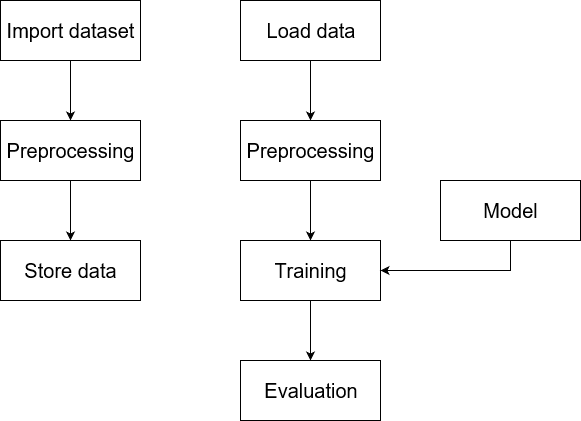
\includegraphics[scale=.4]{figure/block_diag}
	\caption{Framework Pipeline}
	\label{fig:pipeline}
\end{figure}

\section{Signals and Features}
\label{sec:model}

The \textbf{OPPORTUNITY} dataset, succinctly introduced in section \ref{sec:related_work}, has been collected from four subjects accomplishing different Activities of Daily Life (ADLs). As highlighted before, both the subjects and the environment they moved in were meticulously monitored.
The process of acquisition consisted in 5 consecutive runs (named ADL1 to ADL5) that followed a predetermined script, plus a sixth run consisting of 20 repetitions of each of the distinct discrete activity present in the script. Then each vector of samples corresponding to a single time-step is labelled; in the following we'll refer to Task A when we consider an high-level modes of locomotion (\textit{Standing, Walking, Sitting, Lying}) while we'll refer to Task B2 for more specific arm gestures, 17 in total. To these tasks we need of course to add the \textit{Null Class} that we mentioned earlier in this paper: specifically, this label represents the state where the participant does nothing (or something that is not classified among the listed classes). 

The wireless sensors worn by the subjects (IMU - Inertial Measurement Unit) provided acceleration among the three-axes, rate of turn, magnetic field and orientation information; in addition, 12 accelerometers were placed on the subjects' parts of the body sensible to movements (arms, back, hips and feet). All these sensors for a total of 145 distinct acquired channels. \MD{Aggiungere immagine ometti con sensori?}

For the purposes of our work, however, we based the analysis only on on-body sensor signals using just a subset of the available sensors: in this way, we ended up with a total of 113 channels. Another important point is that in the preprocessing phase we performed spline interpolation (which uses a cubic polynomial) in channels that manifested missing data (equivalent to a NaN vale); however, this type of interpolation ends up meaningless if more than the 30\% of data is missing. For this reason we had to discard all the three columns corresponding to one of the physical devices: finally, this led us to work with 110 channels. Since we noticed that the head and tail of the measurement sessions correspond to a transient where most of the sensors are turned-off, we decided to discard them. In this way we ensure that the interpolation phase provides consistent results; the subsequent step consists in normalizing each column with respect to mean and variance. After that, in order to instruct the framework on one subject, we stack sessions from ADL1 to 3 and Drill as a first step to create our training set; then, we assemble also ADL4 and ADL5 to build the test set. 

To conclude the preprocessing phase, finally we decided to follow the same procedure as in several works we cited earlier: we apply in fact the \textit{sliding window} technique on the datasets, obtaining a tensor of windows constituted of \MD{...} samples (\MD{...} ms), using a stride of length \MD{...}. In our case, we decided to assign to each window the most frequent label: this doesn't constitute a problem per se, even when changing the size of the sliding window, as long as it is kept short enough for being representative of a movement.

We found in fact that the choice of window size and stride is fundamental in order to obtain good results: we observed that a window too short can't represent a single gesture with fair precision and, on the contrary, if the window is too large we could include two distinct movements (or modes of locomotion), leading to misplaced classes. The choice of the size of the displacement separating two consecutive windows can guarantee a good trade-off between windows diversity and dataset population.

In the first phase of our project we also tried to create a reduced dataset of features: since each accelerometer returns the acceleration value of in the direction of all the three axes, we tried to substitute these three values with a unique value representing the \textit{mean acceleration} measured by the sensors. In our first experiments, however, this led to poor results: with respect to the simulations where all features were fed to the model, the configuration using the reduced dataset was affected by almost a 5\% loss in terms of accuracy performance. 

\section{Learning Framework}
\label{sec:learning_framework}

One of the main problems in Human Activity Recognition is handling \text{inactivity}.

Thinking of a real recognition system, 
In this paper we compare two different learning strategies, mimicking a real system. In the first \ref{sub:oneshot}, \text{One Shot Classification}, the model is trained to learn a representation of the involved classes together with the null class

\subsection{One Shot Classification}
\label{sub:oneshot}

\subsection{Two Steps Classification}
\label{sub:twosteps}


% !TEX root = template.tex

\section{Results}
\label{sec:results}

As in most of the works mentioned in section \ref{sec:related_work}, besides accuracy, we used $F_1$ measure to estimate the goodness of our models. Defining precision and recall as: 
\begin{equation}
	p = \frac{TP}{TP+FP} \qquad r = \frac{TP}{TP+FN}
\end{equation}
the $F_1$ measure is evaluated as the harmonic average between the two (in the previous formula we have \textit{TP = true positive}, \textit{FP = false positive}, \textit{FN = false negative}). In particular, since we deal with a multi-class problem we need to add a measure of weights to the $F_1$ equation:
\begin{equation}
	F_1 = \sum_i 2w_i \frac{p_i \cdot r_i}{p_i + r_i}
\end{equation} 
where the weights are defined as the number of samples of a particular class divided by the total number of samples $w_i = \frac{n_i}{N}$. The weighted measure can help also with the class imbalance problem that we outlined in the previous section; we must highlight however that our models are still trained on an imbalanced dataset, so in our opinion this could provide only a minor improvement.

In Figures \ref{fig:Anull} and \ref{fig:Anonull} we present the results regarding task A (modes of locomotion, high level movements) for each participant of the experiment: in those configurations we wanted to see if there was one architecture that evidently outperform the others. As we can see, unfortunately that is not the case since among all the frameworks that we tested the differences in terms of weighted $F_1$ measure is negligible. The variation that we can clearly see is among distinct subjects, since they are all studied separately: $S_1$ for example performs better in both the configurations, while $S_2$ is typically the worst. Considering that we consistently performed the same procedure independently from the subject, in this case this discrepancy could be due to a problem occurred during data collection. 

\begin{figure}[ht]
	\centering
	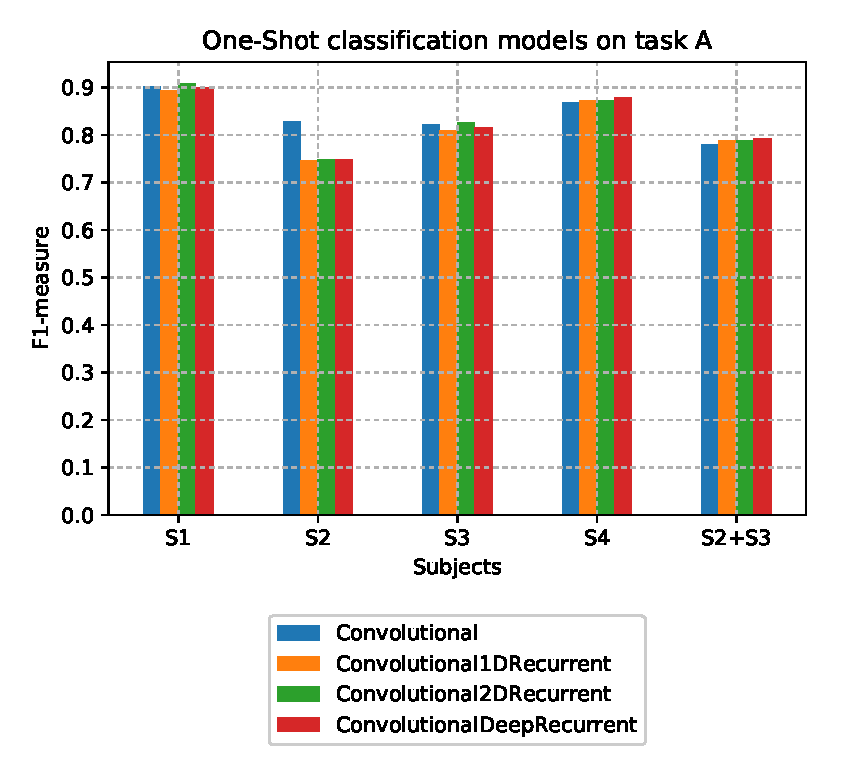
\includegraphics[scale=.4]{figure/A_models_nullclass}
	\caption{Task A : One-Shot Classification}
	\label{fig:Anull}
\end{figure}

With an $F_1$ value of $\sim 0.91$ for the \textit{one-shot} scenario and $\sim 0.94$ in the \textit{two-steps} (if we just consider $S_1$), we can definitely say that the results presented in \cite{Chavarriaga2013} are outperformed by these more powerful deep learning models; with respect to the other subjects, we can say that we obtained state of the art results. In particular it's interesting to see that, when we consider the \textit{Null Class}, the best model with $S_2$ is represented by the neural network with one convolutional layer (Figure \ref{fig:Anull}); when the \textit{Null Class} is discarded, instead, the hybrid model that combines convolutional layers and LSTM provides the best results (Figure \ref{fig:Anonull}). In our opinion the reason is that in certain cases the \textit{Null Class} has to be intended as noise so, when the windows assigned to that class are removed, the LSTM can exploit and reveal the time correlation among different samples more clearly. In addition, we tried to train our architectures on $S_2$ and $S_3$ jointly, using $ADL_4$ and $ADL_5$ of both subjects as test set: as is shown on the last column on the right in Fig \ref{fig:Anull} and \ref{fig:Anonull}, the results are not brilliant. In fact, we obtained a kind of average performance between the results of $S_2$ and $S_3$, in line again with what presented in \cite{Chavarriaga2013}.

\begin{figure}[ht]
	\centering
	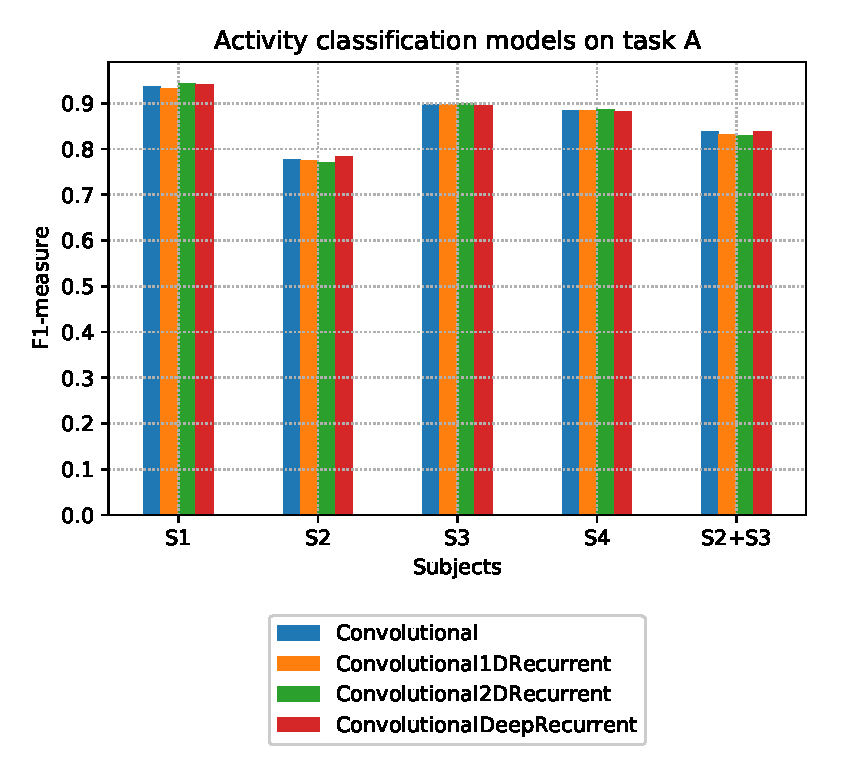
\includegraphics[scale=.4]{figure/A_models_nonullclass}
	\caption{Task A : Two Steps Classification}
	\label{fig:Anonull}
\end{figure}

Finally, as we can see, for task A we can say that using the \textit{two-step} approach definitely helped performances for all users. 

\begin{figure}[ht]
	\centering
	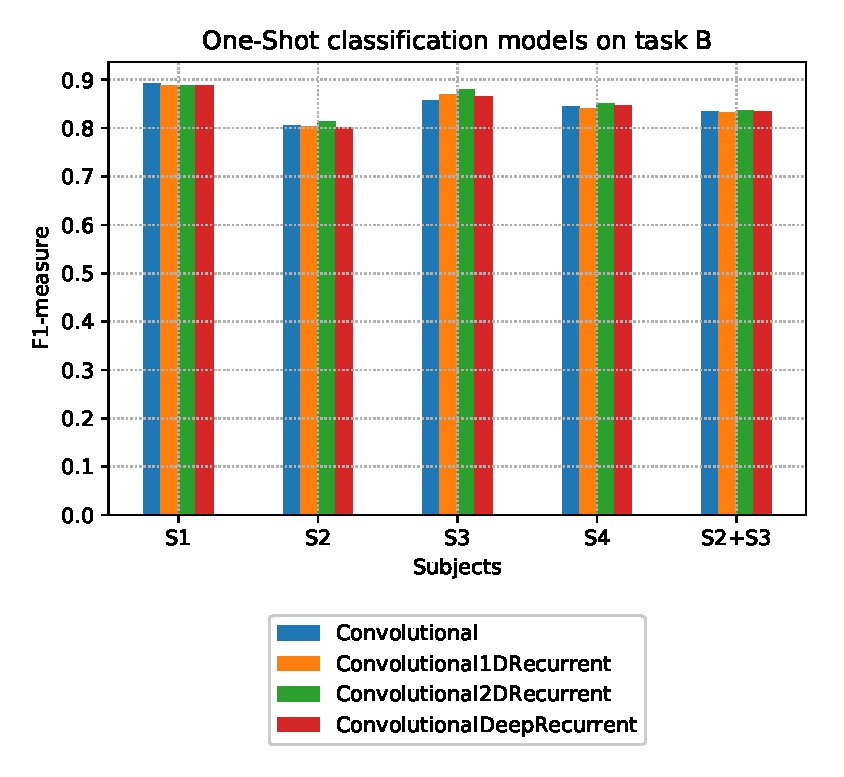
\includegraphics[scale=.4]{figure/B_models_nullclass}
	\caption{Task B : One-Shot Classification}
	\label{fig:Bnull}
\end{figure}

\begin{figure}[ht]
	\centering
	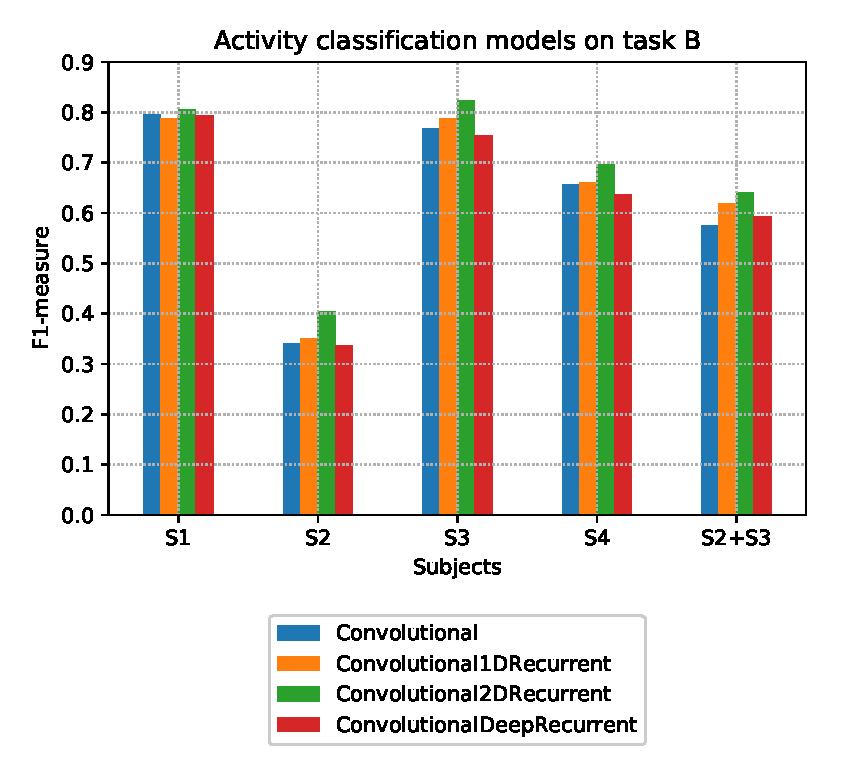
\includegraphics[scale=.4]{figure/B_models_nonullclass}
	\caption{Task B : Two Steps Classification}
	\label{fig:Bnonull}
\end{figure}

% !TEX root = HDA_MDRL.tex

\section{Concluding Remarks}
\label{sec:conclusions}

In our project we realized from scratch two different pipelines to perform activity recognition. A comparison between the two is carried out using different models, which are inspired to the best ones in literature. This helped us understanding that there isn’t a clear best choice from an accuracy point of view; in fact, in locomotion classification, results were slightly worse when the \textit{Null Class} was considered, while in gesture recognition it was the opposite, with a sensible decrease in accuracy when inactivity wasn’t considered. Despite our deep study, still one must examine case by case when to use one model or the other, with respect to the discussion that we developed in section \ref{sec:model}.

Future works could try to implement effectively the Two-Steps classification pipeline, by placing the classification model after the detection one: we tried ourselves, but results weren’t satisfactory enough to be reported here. A good approach to the problem could be trying to understand how the accuracies of the two single models add up when in cascade. In this paper in fact, when comparing the two pipelines, we didn’t keep into account the precision of the detection model in the Two-Step architecture; we considered instead only the classification performances without the null class to provide an estimate of the accuracies achieved using only deep learning models. 

Another thing that is left to be done, is to try to solve the class imbalance problem; a good proposal could be trying to replicate what has been done in \cite{japkowicz2002class}. In our work we only dealt with it for evaluation purposes, but something could be done also to improve the training phase.


\bibliography{biblio}
\bibliographystyle{ieeetr}

\end{document}


